\chapter{Serious Game Stakeholder Experience Assessment Method (SGSEAM) User Guide}
\label{app:sgseam-guide}

This appendix includes the SGSEAM assessment user guide that can be used to guide an assessment to a serious game framework.
  
\section{SGSEAM Overview}
One of the benefits of using a serious game framework is that, if correctly designed, it will 
provide useful and reusable ``building blocks'' with which to develop a variety of serious 
games. Yet how are we to know if a serious game framework has been ``correctly designed''?

Serious Game Stakeholder Experience Assessment Method (SGSEAM) describes a method for 
assessing serious game frameworks from the stakeholder 
experience perspectives.  The goal of SGSEAM is to identify (a) major strengths of a serious game
framework, which aids the community by indicating features of the framework to emulate, and
(b) major shortcomings of the framework, which aids the community by indicating features to avoid.
The benefits of SGSEAM assessment are for the developers of serious game frameworks 
to learn and improve from the findings of the assessment.

SGSEAM is an assessment method instead of an evaluation method. The main purpose 
of an evaluation is to determine the quality of a program by formulating a judgment. An assessment, on 
the other hand, is nonjudgmental. SGSEAM does not try to judge a framework according to a 
standard, or to compare one framework against another. Instead, it is used to identify the major 
strengths and shortcomings of a framework to benefit  the developers of the framework.

\autoref{fig:overview} outlines the steps of the process of applying SGSEAM to a framework.

\begin{figure}[ht!]
  \center
  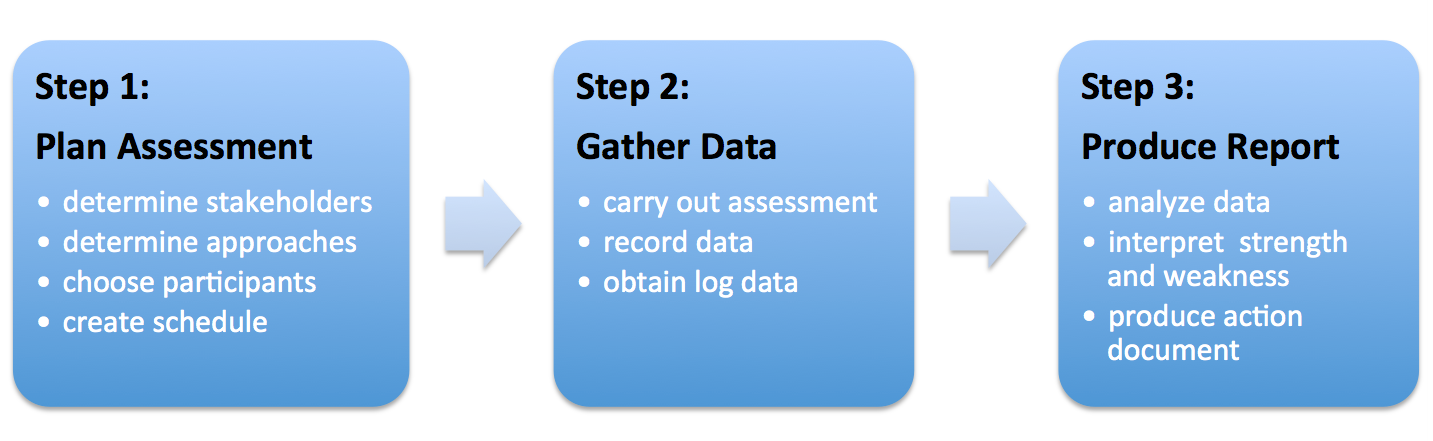
\includegraphics[width=0.8\columnwidth]{sgseam-steps}
  \caption{Applying SGSEAM to a framework}
  \label{fig:overview}
\end{figure}

There are three steps in the process of applying SGSEAM. Step one is to plan the assessment, including
 identifying the stakeholder and participants and creating the assessment plan. The deliverable for this 
 step is the assessment plan document. Step two is to gather data. The deliverable for this step is the 
 assessment data repository. Step three is to produce the strength and weakness report. The deliverable 
 for this step is the action document for framework improvement. The following chapters describe the 
 steps in details.

\section{Plan Assessment}

\subsection{Identify stakeholders}

\begin{shadebox}
\begin{wrapfigure}{l}{0.04\textwidth}
\vspace{-15pt}\hspace{-10pt}
    
\includegraphics[width=0.04\textwidth]{note-icon}
\end{wrapfigure}

Identify the stakeholders in each SGSEAM stakeholder class, write down their names and roles.

\end{shadebox}

SGSEAM assesses the experiences for the stakeholders listed in \autoref{table:stakeholders}. For each 
stakeholder, identify the population, the name and contact if possible. It is important to be able to contact 
the stakeholders in some way, either via email or phone, to get the feedback from their experiences with 
the framework.

\begin{table}[ht!]
  \centering
  \begin{tabular}{|p{0.2\columnwidth}|p{0.4\columnwidth}|p{0.3\columnwidth}|}
    \hline
    \tabhead{Stakeholder class} &
    \tabhead{Definition} &
    \tabhead{Examples} \\
    \hline
    Players &
    participate in the game produced by the framework. &
    students, residents \\
    \hline
    System admins &
    install and maintain the technological game infrastructure. &
    system admin, IT staffs \\
    \hline
    Game designer &
    design the content and game mechanics. &
    instructional designers, content experts \\
    \hline
    Game managers &
    manage the game during the period of game play.&
    sustainability coordinators, residential staffs\\
    \hline
    Game developers &
    develop customization, extend and enhance the game. &
    programmers, internal developers \\
    \hline
  \end{tabular}
  \caption{SGSEAM Stakeholders}
  \label{table:stakeholders}
\end{table}

\subsection{Determine assessment approach}

\begin{shadebox}
\begin{wrapfigure}{l}{0.04\textwidth}
\vspace{-15pt}\hspace{-10pt}
    
\includegraphics[width=0.04\textwidth]{note-icon}
\end{wrapfigure}
Determine the appropriate assessment approaches for each stakeholder.
\end{shadebox}

There are usually multiple assessment approaches for each stakeholder.  \autoref{table:approaches} provides 
an overview of the assessment method and the approaches. The appropriate assessment approaches should 
be determined according to the resource available. The approaches for a stakeholder is additive. The more 
approaches applied, the higher confidence of the assessment can be achieved. 

\begin{table}[ht!]
  \centering
  \begin{tabular}{|p{0.175\columnwidth}|p{0.3\columnwidth}|p{0.43\columnwidth}|}
    \hline
    \tabhead{Stakeholder}&
    \tabhead{Assessment goal}&
    \tabhead{Assessment approaches} \\
    \hline
    Player&
    Determine the extent the framework affect and engage players.&
    	Pre-post effectiveness study(\ref{Pre-Post effectiveness study});\newline
	Self-reported usability metrics(\ref{Self-reported usability metrics});\newline
	Engagement metrics(\ref{Engagement metrics}) \\
    \hline
    System admin&
    Determine strengths and weaknesses in system install and maintenance.&
    	Post-hoc admin interview(\ref{Post-hoc system admin interview});\newline
	In-lab system admin study(\ref{In-lab system admin study}) \\
    \hline
    Game designer&
    Determine strengths and weaknesses in facilitating the game design process.&
    	Post-hoc designer interview(\ref{Post-hoc game designer interview});\newline
	In-lab game design study(\ref{In-lab game design study})\\
    \hline
    Game manager&
    Determine strengths and weaknesses in managing the game.&
    	Post-hoc manager interview(\ref{Post-hoc game manager interview});\newline
	In-lab game management study(\ref{In-lab game management study})\\
    \hline
    Game developer&
    Determine strengths and weaknesses in developing system enhancement.&
    	Post-hoc developer interview(\ref{Post-hoc game developer interview});\newline
	In-lab game development study(\ref{In-lab game development study}) \\
    \hline
  \end{tabular}
  \caption{SGSEAM approaches}
  \label{table:approaches}
\end{table}

The assessment approaches is categorized into in-vivo and in-vitro assessments. The in-vivo approaches, 
such as pre-post test, in-game surveys and post-hoc interviews, assess the real world instance of the game. 
The in-vitro approaches use in-lab experiments in a simulated environment. Different assessment
approaches will have different levels of rigor or validity. For example, the in-lab experiments (in-vitro) can 
enlist several subjects to perform the same pre-defined tasks and collect comparable data in a more 
controlled setting. It is rigor because of the generality achieved from the larger population of
participants under study. On the other hand, in-game surveys or interviews in the in-vivo approach typically 
collect data from different uncontrolled settings with less rigor. But the in-invo data reflect the real world 
interaction between the stakeholders and the framework, thus provides better insights in the real world settings.

The following sections describe in detailed the different approaches for each stakeholder.  Each assessment 
approach describes the goal of the assessment, what data to collect, how to collect the data and how to 
analyze the data to obtain insights about the strengths and weaknesses of the framework from each 
stakeholder's perspective.

\subsection {Choose participants}
\begin{shadebox}
\begin{wrapfigure}{l}{0.04\textwidth}
\vspace{-15pt}\hspace{-10pt}
    
\includegraphics[width=0.04\textwidth]{note-icon}
\end{wrapfigure}
Identify participants from each stakeholder class, Contact them and get consents for their participation.
\end{shadebox}

Once the assessment approaches are determined for each stakeholder class, the next step is to choose participants. 
Identify the  people from the each stakeholder class that may be willing to participate in the assessment, contact them 
and get consents for their participation. 

For example, in the case of pre-post effectiveness study approach for player assessment, this step randomly chooses a 
group of players and present a consent form before the online survey.  In the case of post-hoc game designer interview 
approach, the game designer of a real world game instance of the framework should be identified, contacted and consent 
for the participation in the assessment. When the in-lab game development experiment study is chosen, a group of game 
developers that meet the required development skills of the framework should be identified and contacted.

\subsection{Create assessment plan}
\begin{shadebox}
\begin{wrapfigure}{l}{0.04\textwidth}
\vspace{-15pt}\hspace{-10pt}
    
\includegraphics[width=0.04\textwidth]{note-icon}
\end{wrapfigure}
Create a schedule for each assessment, produce the assessment plan document.
\end{shadebox}

Once we decide what the assessment approaches and who the participants are, the next step is to create the assessment 
schedule and produce the assessment plan document. The document should include the detailed assessment plan for 
each stakeholder class. 

Depends on the assessment approach, the actual tasks of the assessment are different. The player pre-post 
effectiveness study requires the administration of online survey before and after the game. The game designer 
post-hoc interviews requires administration of interviews to the real world game designers of a production 
system. \autoref{figure:assessment-plan} shows an example of the assessment schedule broken down in the tasks 
in the plan document.

\begin{figure}[ht!]
  \centering
  \begin{tabular}{|p{0.5\columnwidth}|p{0.15\columnwidth}|p{0.15\columnwidth}|}
    \hline
    \multicolumn{3}{|c|}{\tabhead{Game design assessment approach: in-lab experiment study}} \\
    \hline
    \tabhead{Task} &
    \tabhead{Estimated Start date} &
    \tabhead{Estimated End date} \\
    \hline
    Design the in-lab experiment instruction & & \\
    \hline
    Ask participants to follow the instruction & & \\
    \hline
    Collect response data from participants & & \\
    \hline
    Obtain log data & & \\
    \hline
    Analyze the data & & \\
    \hline
    Interpret strength and weakness & & \\
    \hline
    Produce action document & & \\
    \hline
  \end{tabular}
  \caption{Assessment schedule in the plan document}
  \label{figure:assessment-plan}
\end{figure}


\section{Gather Data}
This step carries out the assessment, record the data, obtain log data, and refine the assessment plan if necessary. 
The output of this step is a data repository contains all the assessment data that can be analyzed in the next step.

\subsection{Carry out the assessment}
\begin{shadebox}
\begin{wrapfigure}{l}{0.04\textwidth}
\vspace{-15pt}\hspace{-10pt}
    
\includegraphics[width=0.04\textwidth]{note-icon}
\end{wrapfigure}
Carry out the assessment as described in the assessment plan.
\end{shadebox}

For each assessment approach, complete the tasks outlined in the assessment plan, gather the data when carrying out the 
assessment. In the case of game designer post-hoc interview approach, record the interview and take notes if necessary. 
Store all the data into a central data repository. 

In the example of the in-lab game design experiment study, a google form is designed to give detailed step by step 
instructions for the participants to design games using the framework. Participants are asked to record the time they spent completing 
each step and the problems they encountered. They are also asked to provide feedback about their design experiences
in the form of blog posts. 

\subsection{Obtain log data}
\begin{shadebox}
\begin{wrapfigure}{l}{0.04\textwidth}
\vspace{-15pt}\hspace{-10pt}
    
\includegraphics[width=0.04\textwidth]{note-icon}
\end{wrapfigure}
Obtain the log data from the framework, including all the interaction log from the each stakeholder.
\end{shadebox}

Talk to the technical staffs of the framework to find out what kind of log data is available. Obtain the log data in a format that 
is easy to analyze. For example, if the log data is in a database table, ask for the access to the table, or the CSV export of 
the table data. If the log data is in a log file, ask for the access to the file. Store the log data into the central data repository.

\section{Produce Strength and Weakness Report}

This step analyzes all the data gathered from previous steps, interpret the strengths and weakness of the framework, 
and produce the action report regarding to what areas of the framework needs to improve on.

\section{Analyze data}
\begin{shadebox}
\begin{wrapfigure}{l}{0.04\textwidth}
\vspace{-15pt}\hspace{-10pt}
    
\includegraphics[width=0.04\textwidth]{note-icon}
\end{wrapfigure}
Analyze the data from the data repository.
\end{shadebox}
This step performs the data analysis from the data repository obtained from the previous step. For game designer assessment, 
perform queries from user interaction log data to find out the completion time for a certain user interaction task, for instance, the 
time for a game designer to complete the configuration of global game settings. For player assessment, calculate the 
engagement metrics from the game log. For post-hoc interview assessment approach, first transcribe the interview recording into 
text, code and categorize the responses from the interview questions. 

In the example of the in-lab game design experiment study described previously, the assessment data is generalized into 7 tasks
corresponding to distinct types of game design tasks. The time for each task is calculated from the Google form responses. The 
problems reported from the participants are coded and aggregated into the the problems areas. 

\subsection{Interpret strength and weakness}
\begin{shadebox}
\begin{wrapfigure}{l}{0.04\textwidth}
\vspace{-15pt}\hspace{-10pt}
    
\includegraphics[width=0.04\textwidth]{note-icon}
\end{wrapfigure}
Interpret strengths and weaknesses of framework from the data analysis.
\end{shadebox}

From the data analysis step, identified the problem areas which are indicated by having the most reported problems and the 
longest completion time. 

In the example of the in-lab design experiment study, there may be a problem area that had been reported by the most numbers
of participants, and this problem happened in one of the tasks that took the longest time to complete, we could identify a weakness 
area of the framework from the perspective of game designer. If there were no problem reported in some game design tasks and 
the time to complete is short, we could consider those areas are the strengths of the framework.

\subsection{Produce reports with actionable steps}
\begin{shadebox}
\begin{wrapfigure}{l}{0.04\textwidth}
\vspace{-15pt}\hspace{-10pt}
    
\includegraphics[width=0.04\textwidth]{note-icon}
\end{wrapfigure}
Produce the action reports for any improvement identified from the strength and weakness analysis.
\end{shadebox}

Once the strength and weakness of the framework are identified from the data analysis, an action report should be produced. 
This report includes the weakness areas that can be improved and actionable steps on how to improve from 
each stakeholder's perspective. It also includes the strength areas that the framework needs to maintain.

By producing the report with actionable steps to improve the framework, the SGSEAM assessment is completed.  
